\section{Experiment}

\subsection{Output voltage of a voltage source}

\begin{figure}[H]
	\centering
	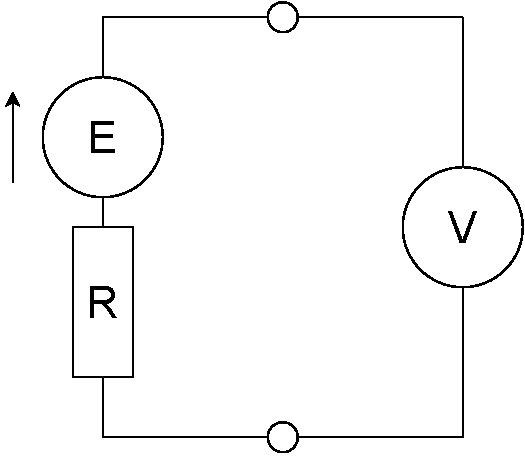
\includegraphics[width=5cm]{schematics/analog_voltage.pdf}
	\caption{Voltage measurement schematic}
	\label{fig:voltage_schematics}
\end{figure}

\subsubsection*{Analog measurement}

For analogue measurements we used an LM-3 meter, characterized by an accuracy class of 0.5 and an internal resistance of \SI{1}{\frac{\kilo\ohm}{\volt}}.

\begin{table}[H]
	\centering
	\begin{tabular}{ c | c | c | c | c | c | c | c}
		$R_c [\unit{\ohm}]$ & $\alpha$ & $\alpha_{max}$  & $V_r [\unit{\volt}]$ & $V [\unit{\volt}]$ & $\Delta V [\unit{\volt}]$ & $\delta V  \unit{\percent}$ & $V \pm \Delta V [\unit{\volt}]$\\
		\hline
		0 & 40 & 75 & 7.5 & 4.0 & 0.037500 & 0.937500 & $4.00 \pm 0.04$\\
		\hline
		10 & 40 & 75 & 7.5 & 4.0 & 0.037500 & 0.937500 & $4.00 \pm 0.04$\\
		\hline
		100 & 39.5 & 75 & 7.5 & 3.95 & 0.037500 & 0.949367 & $3.95 \pm 0.04$\\
		\hline
		1000 & 35 & 75 & 7.5 & 3.5 & 0.037500 & 1.071429 & $3.50 \pm 0.04$\\
		\hline
		5000 & 56 & 75 & 0.15 & 0.112 & 0.000750 & 0.669643 & $0.1120 \pm 0.0008$\\
		\hline
		10000 & 30 & 75 & 0.15 & 0.06 & 0.000750 & 1.250000 & $0.0600 \pm 0.0008$
	\end{tabular}
	\caption{Analog voltage measurement for $E \sim \SI{3.9}{\volt}$ ($R_c$ -- circuit resistance, $\alpha$ -- actual needle swing, $\alpha_{max}$ -- maximal swing, $V_r$ -- range, $V$ -- calculated voltage, $\Delta V$ -- absolute error, $\delta V$ -- relative error)}
	\label{tab:analog_volt_1}
\end{table}

\begin{table}[H]
	\centering
	\begin{tabular}{ c | c | c | c | c | c}
		$R_v [\unit{\ohm}]$  & $\Delta_m V [\unit{\volt}]$ & $\delta_m V $ & $c [\unit{\volt}]$ & $V_c [\unit{\volt}]$ & $V_c \pm \Delta V [\unit{\volt}]$\\
		\hline
		7500 & 0 & 0 & 0 & 4 & 4.00 +- 0.04\\
		\hline
		7500 & -0.005333 & -0.001332 & 0.005333 & 4.005333 & $4.01 \pm  0.04$\\
		\hline
		7500 & -0.052667 & -0.013158 & 0.052667 & 4.002667 & $4.01 \pm 0.04$\\
		\hline
		7500 & -0.466667 & -0.117647 & 0.466667 & 3.966667 & $3.97 \pm 0.04$\\
		\hline
		150 & -3.733333 & -0.970874 & 3.733333 & 3.845333 & $3.8453 \pm 0.0008$\\
		\hline
		150 & -4 & -0.985222 & 4 & 4.06 & $4.0600 \pm 0.0008$
	\end{tabular}
	\caption{Analog voltage measurement for $E \sim \SI{3.9}{\volt}$ ($R_v$ -- internal voltmeter resistance, $\Delta_m V$ -- systematic error, $\delta_m V$ -- ?, $c$ -- correction factor, $V_c$ -- ?}
	\label{tab:analog_volt_2}
\end{table}

Example calculations for $R_c = \SI{100}{\ohm} $ are shown in Equations~\ref{eq:analog_V},~\ref{eq:analog_Delta_V},~\ref{eq:analog_delta_V},~\ref{eq:analog_R_v},~\ref{eq:analog_Delta_m},~\ref{eq:analog_delta_m},~\ref{eq:analog_c},~\ref{eq:analog_V_c}.

\begin{equation}
	 V = \frac{\alpha\cdot V_{r}}{\alpha_{max}} = \frac{39.5\cdot \SI{7.5}{\volt}}{75} = \SI{3.95}{\volt}
	 \label{eq:analog_V}
\end{equation}

\begin{equation}
	\Delta V = \frac{V_{r}\cdot cl}{100\unit{\percent}} = \frac{\SI{7.5}{\volt}\cdot 0.5\unit{\percent}}{100 \unit{\percent}} = \SI{0.0375}{\volt}
	\label{eq:analog_Delta_V}
\end{equation}

\begin{equation}
	  \delta V = \frac{\Delta V}{V}\cdot 100\unit{\percent} = \frac{0.0375}{3.95}\cdot 100\unit{\percent} \approx 0.949367\unit{\percent}
	  \label{eq:analog_delta_V}
\end{equation}

\begin{equation}
	R_v = V_r\cdot \SI{1}{\frac{\kilo\ohm}{\volt}} = \SI{7.5}{\volt}\cdot \SI{1000}{\frac{\ohm}{\volt}} = \SI{7500}{\ohm}
	\label{eq:analog_R_v}
\end{equation}

\begin{equation}
	\Delta_m V = -V\cdot\frac{R_c}{R_v} = -\SI{3.95}{\volt}\cdot\frac{\SI{100}{\ohm}}{\SI{7500}{\ohm}} \approx -\SI{0.052667}{\volt}
	\label{eq:analog_Delta_m}
\end{equation}

\begin{equation}
	\delta_m V = -\frac{R_c}{R_c + R_v} = -\frac{\SI{100}{\ohm}}{\SI{100}{\ohm} + \SI{7500}{\ohm}} \approx -0.013158
	\label{eq:analog_delta_m}
\end{equation}

\begin{equation}
	c = -\Delta_m V = -(-\SI{0.052667}{\volt}) = \SI{0.052667}{\volt}
	\label{eq:analog_c}
\end{equation}

\begin{equation}
	V_c = V + c = \SI{3.95}{\volt} + \SI{0.052667}{\volt} = \SI{4.002667}{\volt}
	\label{eq:analog_V_c}
\end{equation}


\subsubsection*{Digital measurement}

\begin{table}[H]
	\centering
	\begin{tabular}{ c | c |  c | c | c | c | c}
		$R_c [\unit{\ohm}]$  & Accuracy & $V_r [\unit{\volt}]$ & $V [\unit{\volt}]$ & $\Delta V [\unit{\volt}]$ & $\delta V [\unit{\percent}]$ & $V \pm \Delta V [\unit{\volt}]$ \\
		\hline
		0  & $0.0035 \pm 0.0005$ & 10 & 3.9996 & 0.000190 & 0.004750 & 3.9996 +- 0.0002\\
		\hline
		10  & $0.0035 \pm 0.0005$  & 10 & 3.99953 & 0.000190 & 0.004750 & 3.9995 +- 0.0002\\
		\hline
		100  & $0.0035 \pm 0.0005$  & 10 & 3.99964 & 0.000190 & 0.004750 & 3.9996 +- 0.0002\\
		\hline
		1000 &$0.0035 \pm 0.0005$  & 10 & 3.99931 & 0.000190 & 0.004750 & 3.9993 +- 0.0002\\
		\hline
		5000  & $0.0035 \pm 0.0005$  & 10 & 3.99791 & 0.000190 & 0.004752 & 3.9979 +- 0.0002\\
		\hline
		10000 & $0.0035 \pm 0.0005$  & 10 & 3.99593 & 0.000190 & 0.004751 & 3.9959 +- 0.0002\\
	\end{tabular}
	\caption{Digital voltage measurement for $E \sim \SI{3.9}{\volt}$ ($R_c$ -- circuit resistance, Accuracy: $\pm$ (a$\unit{\percent}$ of reading + b$\unit{\percent}$ of range), $V_r$ -- range, $V$ -- measured voltage, $\Delta V$ -- absolute error, $\delta V$ -- relative error)}
	\label{tab:digital_voltage_1}
\end{table}

\begin{table}[H]
	\centering
	\begin{tabular}{  c | c | c | c | c | c}
		 $R_v [\unit{\mega\ohm}]$ & $\Delta_m V [\unit{\volt}]$ & $\delta_m V$ & $c [\unit{\volt}]$ & $V_c [\unit{\volt}]$ & $V_c \pm \Delta V [\unit{\volt}]$\\
		\hline
		10 & 0 & 0 & 0 & 3.9996 & 3.9996 +- 0.0002\\
		\hline
		10 & -0.000003 & -0.000001 & 0.000004 & 3.999534 & 3.9995 +- 0.0002\\
		\hline
		10 & -0.000040 & -0.000010 & 0.000040 & 3.999680 & 3.9997 +- 0.0002\\
		\hline
		10 & -0.000400 & -0.000100 & 0.000400 & 3.999710 & 3.9997 +- 0.0002\\
		\hline
		10 & -0.001999 & -0.000500 & 0.001999 & 3.999909 & 3.9999 +- 0.0002\\
		\hline
		10 & -0.003996 & -0.000999& 0.0039969 & 3.999926 & 3.9999 +- 0.0002\\
	\end{tabular}
	\caption{Digital voltage measurement for $E \sim \SI{3.9}{\volt}$ ($R_v$ -- internal voltmeter resistance, $\Delta_m V$ -- systematic error, $\delta_m V$ -- ?, $c$ -- correction factor, $V_c$ -- ?}
	\label{tab:digital_voltage_2}
\end{table}

Example calculations for $R_c = \SI{5000}{\ohm}$ are shown in Equations~\ref{eq:digital_Delta_V},~\ref{eq:digital_delta_V},~\ref{eq:digital_Delta_m},~\ref{eq:digital_delta_m},~\ref{eq:digital_c},~\ref{eq:digital_V_c}.

\begin{equation}
	\begin{split}
		\Delta V &= \frac{a}{100\unit{\percent}}\cdot V + 	\frac{b}{100\unit{\percent}}\cdot V_r = \frac{0.0035\unit{\percent}}{100\unit{\percent}}\cdot\SI{3.99791}{\volt} + \frac{0.0005\unit{\percent}}{100\unit{\percent}}\cdot\SI{10}{\ohm} =\\
		&= \SI{0.00014}{\volt} + \SI{0.00005}{\volt} = \SI{0.00019}{\volt}
	\end{split}
	\label{eq:digital_Delta_V}
\end{equation}

\begin{equation}
	\delta V = \frac{\Delta V}{V}\cdot 100\unit{\percent} = \frac{\SI{0.00019}{\volt}}{\SI{3.99791}{\volt}}\cdot 100\unit{\percent} = 0.004752\unit{\percent}
	\label{eq:digital_delta_V}
\end{equation}

\begin{equation}
	\Delta_m V = -V\cdot\frac{R_c}{R_v} = -\SI{3.99791}{\volt}\cdot\frac{\SI{5000}{\ohm}}{\SI{10000000}{\ohm}} \approx -\SI{0.001999}{\volt}
	\label{eq:digital_Delta_m}
\end{equation}

\begin{equation}
	\delta_m V = -\frac{R_c}{R_c + R_v} = -\frac{\SI{5000}{\ohm}}{\SI{5000}{\ohm} + \SI{10000000}{\ohm}} \approx -0.000500
	\label{eq:digital_delta_m}
\end{equation}

\begin{equation}
	c = -\Delta_m V = -(-\SI{0.001999}{\volt}) = \SI{0.001999}{\volt}
	\label{eq:digital_c}
\end{equation}

\begin{equation}
	V_c = V + c = \SI{3.99791}{\volt} + \SI{0.001999}{\volt} = \SI{3.999909}{\volt}
	\label{eq:digital_V_c}
\end{equation}


\subsection{Voltage divider}